\documentclass[border=10pt]{standalone}

\usepackage{tikz}
\usepackage{tikzsymbols}
\usetikzlibrary{calc,patterns,shapes.geometric}

\def\centerarc[#1](#2)(#3:#4:#5){\draw[#1] ($(#2)+({#5*cos(#3)},{#5*sin(#3)})$) arc (#3:#4:#5);}

\begin{document}
	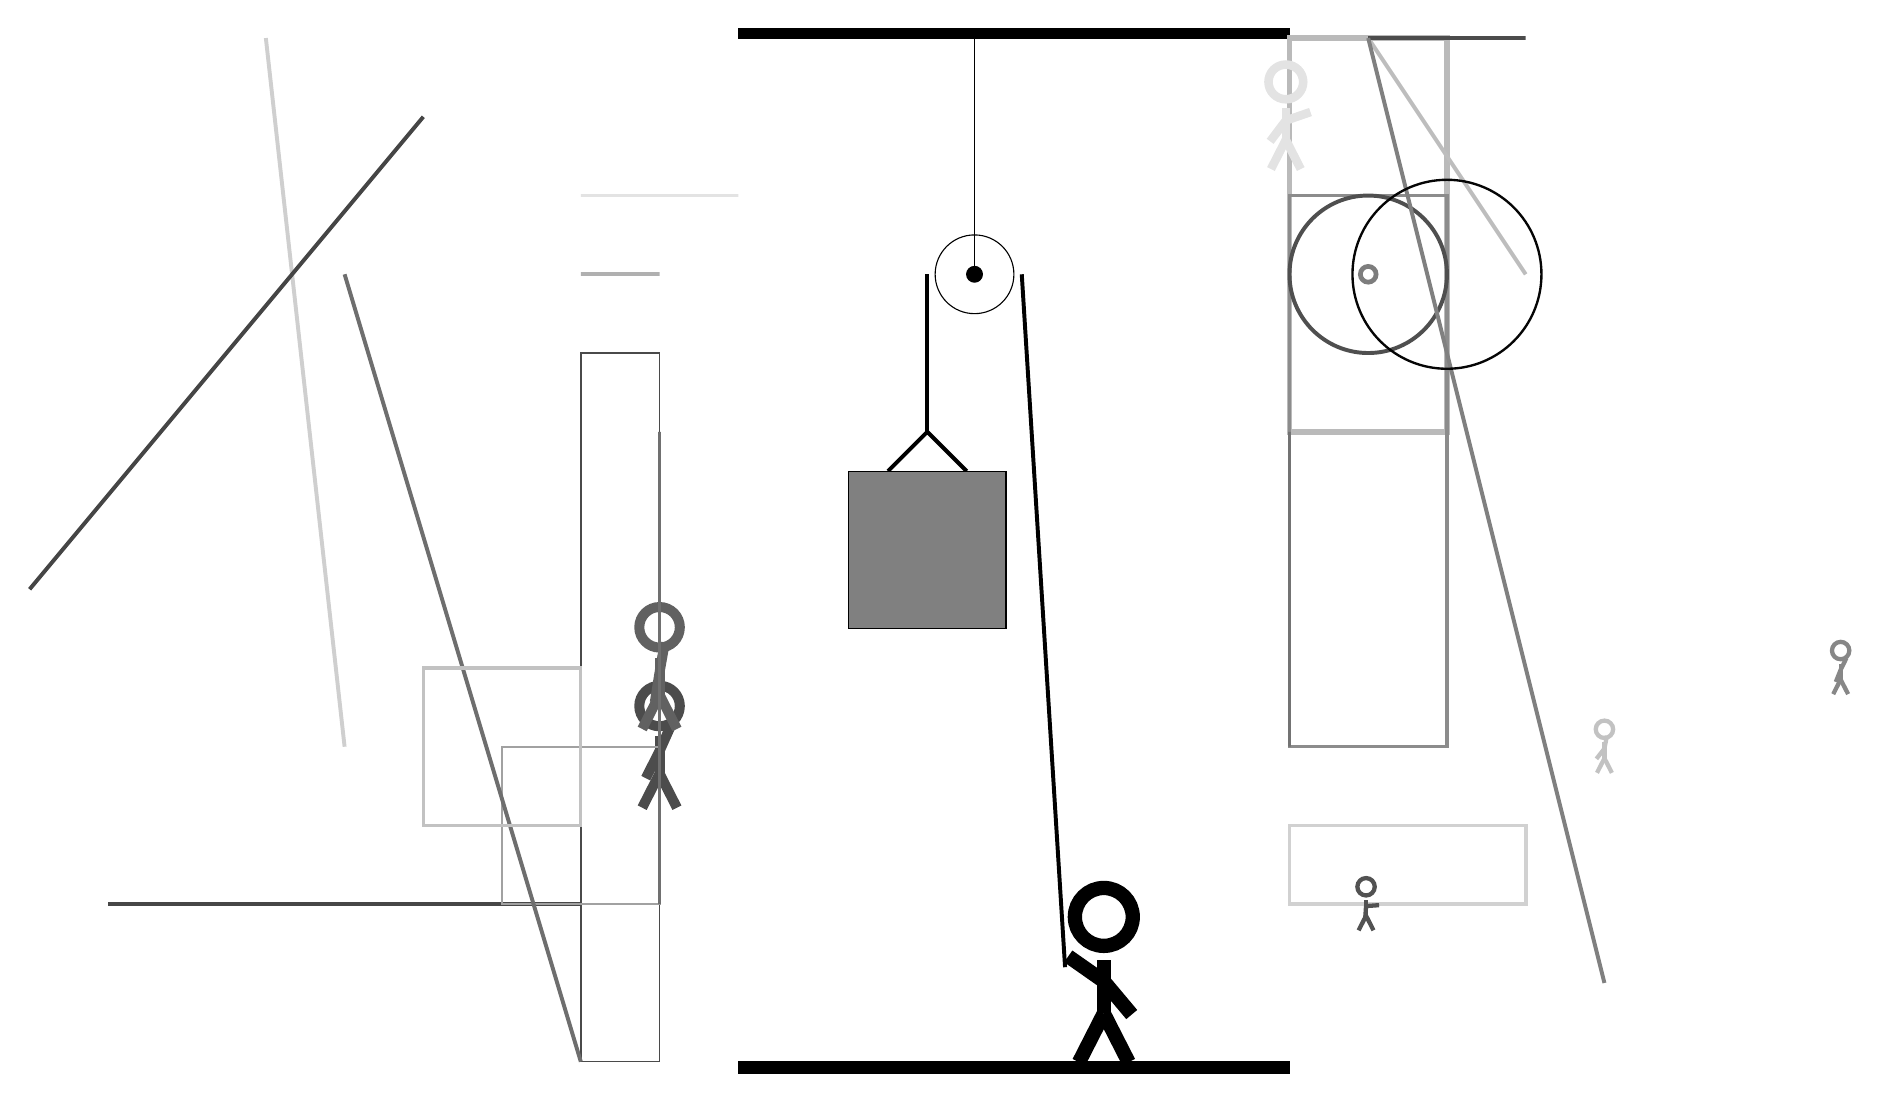
\begin{tikzpicture}
		%%%%% START %%%%%
		
		\draw[fill=black] (-2, 10) rectangle (5, 10.125);
		
		\draw (1, 7) circle (0.5);
		\draw[fill=black] (1, 7) circle (0.1);
		\draw (1, 10) -- (1, 7);
		
		\node[line width=0.6mm, color=black!70] at (-3, 1) {\Strichmaxerl[7][63][66]};
		
		\draw[line width=0.7mm, color=black!27] (7, 10) rectangle (5, 5);
		\draw[line width=0.2mm, color=black!71] (-3, 6) rectangle (-4, -3);
		\draw[line width=0.5mm, color=black!18] (5, -1) rectangle (8, 0);
		\node[line width=0.6mm, color=black!24] at (9, 1) {\Strichmaxerl[3][52][79]};
		\draw [line width=0.6mm, color=black!51](6, 7) circle (0.1);
		
		\node[line width=0.2mm, color=black!11] at (5, 9) {\Strichmaxerl[6][53][19]};
		\draw[line width=0.5mm, color=black!72](-4, -1) -- (-10, -1);
		\draw[line width=0.5mm, color=black!31] (-3, 7) rectangle (-4, 7);
		\draw[line width=0.4mm, color=black!45] (7, 8) rectangle (5, 1);
		\node[line width=0.6mm, color=black!68] at (6, -1) {\Strichmaxerl[3][86][4]};
		\node[line width=0.7mm, color=black!47] at (12, 2) {\Strichmaxerl[3][68][64]};
		\draw[line width=0.5mm, color=black!26](6, 10) -- (8, 7);
		\draw[line width=0.5mm, color=black!19](-7, 1) -- (-8, 10);
		\draw [line width=0.5mm, color=black!69](6, 7) circle (1.0);
		\draw[line width=0.3mm, color=black!37] (-3, 1) rectangle (-5, -1);
		\draw[line width=0.5mm, color=black!70] (6, 10) rectangle (8, 10);
		\node[line width=0.5mm, color=black!62] at (-3, 2) {\Strichmaxerl[7][81][80]};
		\draw[line width=0.5mm, color=black!50](6, 10) -- (9, -2);
		\draw[line width=0.3mm, color=black!56] (-3, -1) rectangle (-3, 5);
		\draw[line width=0.4mm, color=black!11] (-4, 8) rectangle (-2, 8);
		
		\draw[line width=0.5mm, color=black!73](-6, 9) -- (-11, 3);
		\draw[line width=0.5mm, color=black!57](-4, -3) -- (-7, 7);
		\draw[line width=0.4mm, color=black!24] (-4, 2) rectangle (-6, 0);
		\draw[line width=0.4mm, color=black!55] (5, 5) rectangle (5, 1);
		
		\draw [line width=0.3mm, color=black!98](7, 7) circle (1.2);
		
		\draw[line width=0.5mm] (-0.1, 4.5) -- (0.4, 5.0) -- (0.9, 4.5);
		\draw[fill=black!50] (-0.6, 4.5) rectangle (1.4, 2.5);
		
		\draw[line width=0.5mm] (0.4, 7) -- (0.4, 5.0);
		\centerarc[line width=0.5mm](1, 7)(0:180:0.6);
		\draw[line width=0.5mm](1.6, 7) -- (2.15, -1.8);
		
		\node at (2.6, -1.9) {\Strichmaxerl[10][-35][-50]};
		
		\draw[fill=black] (-2, -3) rectangle (5, -3.15);
		
		%%%%% END %%%%%
	\end{tikzpicture}
\end{document}